\documentclass[twoside,12pt]{article}
\usepackage{eepic}
\usepackage[dvips]{epsfig}
% \usepackage{epic}
% \usepackage{makeidx}
\setlength\textheight{43\baselineskip}
\setlength\textwidth{414pt}
\setlength\topmargin{+27pt}
\newlength{\temporary}
\setlength\temporary{\paperwidth}
\addtolength\temporary{-\textwidth}
\addtolength\temporary{-2.5in}
\setlength\oddsidemargin{\temporary}
\setlength\evensidemargin{0.25in}

% \makeindex
\title{Lanczos eigensolver for complex Hermitian systems}
\author{Copyright \copyright 2002\\
E. Robert Tisdale, Fabiano Oyafuso, Hook Hua, and Gerhard Klimeck}
\begin{document}
% \pagenumbering{roman}
\bibliographystyle{plain}
\maketitle

\begin{abstract}
A parallel eigensolver designed to find a few eigenvalues and, optionally,
their corresponding eigenvectors in a sparse complex Hermitian matrix
with up to $10^{8}$ diagonal elements using Lanczos' algorithm
has been implemented in the ANSI/ISO C computer programming language
using the Message Passing Interface (MPI) standard to complement
the eigensolvers provided in the Parallel ARnoldi PACKage (PARPACK).
The eigensolver runs on Beowulf clusters at the 
Jet Propulsion Laboratory (JPL).
The package is open source software and is distributed
under the terms of the GNU Lesser General Public License (LGPL)
on the Internet through the Open Channel Foundation at
{\tt http://www.openchannelsoftware.com/}.
\end{abstract}

\section{Introduction}
The NanoElectronic MOdeling (NEMO) software package developed here
at the Jet Propulsion Laboratory (JPL) over the last several years
required an eigensolver for large sparse complex Hermitian matrices.
JPL scientists were obliged to implement the eigensolver themselves
for Beowulf clusters using Lanczos' algorithm, because, at the time,
there were no suitable parallel Lanczos eigensolvers
for large sparse complex Hermitian matrices.
The most widely used parallel eigensolver was PARPACK\cite{ARPACK, www:arpack}.
% \cite{www:arpack}.
However, for complex matrices, PARPACK implements only Arnoldi, which
does not utilize the Hermiticity of the linear operator in question.
It was found that for our purposes, PARPACK was a bit slow 
and consumed too much memory (typical memory requirements 
for storage of the matrix alone is $\sim 10-100$ GB).
The Lanczos eigensolver developed to accommodate these needs
is faster and requires less memory than the available parallel 
Arnoldi eigensolvers for large sparse complex Hermitian matrices.
However, no effort has been made to make the algorithm as robust
as other publicly available solvers; in effect, 
some robustness has been sacrificed in favor of speed.
For example, orthogonality of the resulting eigenvectors must be 
checked manually, and degeneracies of the eigenvalues must be deduced 
from the underlying physical problem.
Also, no guarantee is made as to \emph{which} eigenvalues within
a range will be computed, so that computation of all desired
eigenvalues may require insight into the system being modeled.
Thus, the JPL NEMO Lanczos eigensolver software package
is intended to complement existing parallel eigensolvers such as those 
distributed with PARPACK as indicated in the table below.
%
\begin{center}
\begin{tabular}{r|ll|ll}
	&Arnoldi	&		&Lanczos	&		\\
\hline
real	&non-symmetric	&(PARPACK)	&symmetric	&(PARPACK)	\\
complex	&non-Hermitian	&(PARPACK)	&Hermitian	&(JPLNEMO)
\end{tabular}
\end{center}
%
In this work, we describe the implemented algorithm (section~\ref{sec:alg})
and its API (section~\ref{sec:api}).  In section~\ref{sec:cmp},
we discuss benchmarking results for a single test problem.  
The appendices include installation instructions as well
as a description of the Nemo Math Library (NML), which contains
definitions of several basic mathematical data structures used in
the package.

\section{The Lanczos algorithm}\label{sec:alg}
The Lanczos algorithm is a well-known iterative algorithm
which reduces a complex Hermitian matrix $A$
to a real symmetric tridiagonal matrix
\begin{equation}\label{basic_lancz}
T_{n} = Q_{n}^{*}AQ_{n}
\end{equation}
where the columns $\{q_{j}\}$ of
\begin{equation}
Q_{n} = \left[q_{1}|q_{2}|\cdots|q_{n}\right]
\end{equation}
constitute an orthonormal basis for the $n$-dimensional Krylov subspace 
at iteration $n$.
The real symmetric tridiagonal matrix is given by
\begin{equation}
T_{n} = \left[
\begin{array}{rrrrrrr}
\alpha_{1}&\beta_{1} &   &   &   &   &   \\
 \beta_{1}&\alpha_{2} &\beta_{2} &   &   &   &   \\
&\beta_{2} & . & . &   &   &   \\
   &   & . & . & . &   &   \\
   &   &   & . & . &\multicolumn{1}{l}{.} &   \\
   &   &   &   & . &\alpha_{n\!-\!1}&\beta_{n\!-\!1} \\
   &   &   &   &   &\beta_{n\!-\!1} &\alpha_{n}
\end{array}
\right]
\end{equation}
where both the diagonal elements $\alpha_{n}$
and off-diagonal elements $\beta_{n}$ are computed at iteration $n$.

Beginning with $q_{0} = 0$, $r_{0} \neq 0$ and $\beta_{0} = ||r_{0}||$,
at iteration $n$
\begin{eqnarray} \label{lancz_alg}
     q_{n} &\leftarrow& r_{n\!-\!1}/\beta_{n\!-\!1}	\nonumber	\\
     r_{n} &\leftarrow& Aq_{n}				\nonumber	\\
\alpha_{n} &\leftarrow& q_{n}^{*}r_{n}			\nonumber	\\
     r_{n} &\leftarrow& r_{n} - \beta_{n\!-\!1}q_{n\!-\!1} - \alpha_{n}q_{n}
							\nonumber	\\
 \beta_{n} &\leftarrow& ||r_{n}||
\end{eqnarray}
The choice of $r_{0}$ is not completely arbitrary and
the best choice will depend upon matrix $A$.

In Eq.(\ref{lancz_alg}), the user is required to supply his or her own
parallelized matrix-vector multiplication.  The temporary vectors $q_j$ 
and $r_j$ are distributed in a user-defined fashion.
Since the intent is to run the algorithm on very large systems, memory
limitations necessitate that these temporary vectors not be stored.
If eigenvectors as well as eigenvalues need to be computed,
the algorithm must be restarted from scratch once the eigenvalues are computed.

Rewriting Eq.(\ref{basic_lancz}) as follows 
\begin{eqnarray}\label{basic_lancz_meaning}
T_{n} 
&=& Q_{n}^{*}AQ_{n} \nonumber \\
&=& Q_n^* (Q_n Q_n^* A) Q_n
\end{eqnarray}
demonstrates that the symmetric tridiagonal matrix $T_n$ 
is merely the orthogonal projection of $A$ onto the space spanned 
by $K_n = \{ q_1, ..., q_n \}$ written in terms of the basis $K_n$.
The eigenvalues (Ritz values) of $T_n$, then, 
are approximations to those of $A$.
Algorithm (\ref{lancz_alg}) iterates until the requested number of
eigenvalues have converged according to a stopping criterion that
specifies the tolerated change in eigenvalues from one iteration to the next.
However, since the algorithm used ({\tt subroutine dstebz} from LAPACK) 
to determine eigenvalues of $T_n$ takes $\mathcal{O}(n^2)$ time, it 
is impractical to solve for the eigenvalues of $T_n$ for all 
positive integers $n$.  Instead, the eigenvalues of $T_n$ are
computed with a frequency specified by the user.

Once a convergence criterion has been achieved and an eigenvalue $E$
determined, eigenvectors of $T_n$ corresponding to $E$ can be computed.
\begin{eqnarray}
T_{n} \Psi &=& E \Psi
\end{eqnarray}
Premultiplying $T_n = Q_{n}^{*}AQ_{n}$ by $Q_n$ gives
\begin{eqnarray}
A (Q_n \Psi) &=& E (Q_n \Psi)
\end{eqnarray}
One sees that $Q_n \Psi$ is an eigenvector of $A$.  
However, since $Q_n$ is not stored due to (anticipated) limited
storage, the computation must restarted from scratch to compute
the eigenvectors of $A$ associated with the Ritz value $E$.

\section{The Application Program Interface (API)}\label{sec:api}
In this section we describe the API associated with the Lanczos eigensolver.  
A demonstration of its use is contained in the \verb!examples! directory
of the distribution.
There are two principal function calls at the user's disposal:
\begin{enumerate}
\item	{\tt eigenvaluesLanczos} (computes eigenvalues)
\item	{\tt eigenvectorsLanczos} (computes the corresponding eigenvectors)
\end{enumerate}
Both functions require the application program to provide
a matrix-vector multiplier \\
\\
{\tt void matmul(const~int*~argument[], nml\_dcscalar*~pw, const~nml\_dcscalar*~pv);} \\
\\
to compute $w \leftarrow Av$ where
{\tt pv} is a pointer to the first element of complex  input vector $v$,
{\tt pw} is a pointer to the first element of complex output vector $w$
and the representation of matrix $A$ depends upon the user implementation.
An array of pointers {\tt argument} to built-in type {\tt int}
may be used to pass optional arguments to the matrix-vector multiplier.
The data type {\tt nml\_dcscalar}, essentially a double precision
complex float, is an instance of a class of data structures defined
by the JPL NEMO math library described in further detail in 
appendix~\ref{app:nml}.
% \pagebreak
The first function
\begin{verbatim}
nml_extent eigenvaluesLanczos(  /* number of eigenvalues actually found */
    nml_dvector  *value,        /*   out real eigenvalue vector         */
    nml_d3bands  *T,            /*   out symmetric tridiagonal matrix   */
    nml_extent   *pIterations,  /*   out actual number of iterations    */
    nml_dcvector *r_n,          /* inout r_{n} = q_{n+1}*beta_{n}       */
    nml_dcvector *q_n,          /* inout current  complex Lanczos vector*/
    nml_dcvector *q_n1,         /* inout previous complex Lanczos vector*/
    nml_extent   length,        /* in extent of vectors r_n, q_n & q_n1 */
    nml_extent   requested,     /* in requested number of eigenvalues   */
    int ConvCheckStartIter,     /* in convergence check start iteration */
    int ConvCheckSkipRate,      /* in convergence check skip rate       */
    nml_extent   imax,          /* in maximum number of iterations + 1  */
    nml_dscalar  emin,          /* in eigenvalue search lower bound     */
    nml_dscalar  emax,          /* in eigenvalue search upper bound     */
    nml_dscalar  tolerance,     /* in eigenvalue convergence tolerance  */
    nml_dscalar  resolution,    /* in eigenvalue separation minimum     */
    void (*matmul)(const int**, nml_dcscalar*, const nml_dcscalar*),
    const int*   argument[],    /* matrix-vector multiply argument list */
    FILE         *fp_trace,     /* in   trace log text file pointer     */
    FILE         *fp_instant,   /* in instant log text file pointer     */
    FILE         *fp_log,       /* in message log text file pointer     */
    int          verbose        /* in verbose diagnostic messages       */
    );
\end{verbatim}
%     nml_extent   nsuc,          /* in maximum number no success         */
%     nml_dscalar  shift,         /* in eigenvalue shift                  */
returns the number of eigenvalues between {\tt emin} and {\tt emax}
actually found for the Hermitian operator specified by {\tt matmul}
up to the number of eigenvalues requested.
The application should request no more eigenvalues
than the maximum number of iterations $\mbox{{\tt imax}} - 1$.

Memory must be pre-allocated for the real eigenvalue vector
% \begin{minipage}{\textwidth}
% \vspace{5mm}
% \hspace{10mm}
\begin{verbatim}
nml_dvector* value = nml_dv_new(imax);
\end{verbatim}
% \end{minipage}
and the real symmetric tridiagonal matrix
\begin{verbatim}
nml_d3bands* T = nml_d3_new(imax);
\end{verbatim}
where {\tt imax} is actually one greater than
the maximum number of Lanczos iterations.
The actual number of iterations required
is returned in the {\tt nml\_extent} to which {\tt pIterations} points.

Memory must be pre-allocated for complex vector
\begin{verbatim}
nml_dcvector* q_n = nml_dcv_new(length);
\end{verbatim}
and preallocated and initialized for complex vectors
\begin{verbatim}
nml_dcvector* r_n = nml_dcv_fill(nml_dcv_new(length), nml_dcmplx(1.0, 0.0));
\end{verbatim}
and
\begin{verbatim}
nml_dcvector* q_n1 = nml_dcv_fill(nml_dcv_new(length), nml_dcmplx(0.0, 0.0));
\end{verbatim}
where {\tt length} is the extent of the segment
of vectors $q_{n}$, $r_{n}$ and $q_{n\!-\!1}$ on each processor.

Four additional arguments
\begin{center}
\begin{tabular}{l|c|c}
			& suggested	&lower	\\
argument		& value		&bound	\\
\hline
{\tt ConvCheckStartIter}&$100$		&$0$	\\
{\tt ConvCheckSkipRate}	&$100$		&$1$	\\
\hline
%{\tt nsuc}		&{\tt imax}	&$1$	\\
%\hline
{\tt tolerance}		&$10^{-8}$	&$0$	\\
{\tt resolution}	&$10^{-6}$	&$0$
%{\tt shift}		&$0$
\end{tabular}
\end{center}
steer the Lanczos iteration.
To reduce computational expense, eigenvalues for the real symmetric 
tridiagonal matrix $T_{n}$ are computed starting with the iteration
number specified by {\tt ConvCheckStartIter} and at intervals of 
{\tt ConvCheckSkipRate}.
The Fortran~77 {\tt subroutine dstebz} from the Linear Algebra PACKage (LAPACK)
is used for the computation.
Eigenvalues differing from the previously calculated eigenvalues
by less than {\tt tolerance} are said to have converged.
The eigenvalue convergence tolerance must be a positive number
and should probably be larger than the expected numerical error
in the largest desired eigenvalue.
Within a given iteration, the solver discards any eigenvalue 
separation of less than {\tt resolution} to eliminate computed degeneracies.
The eigenvalue resolution should not be negative,
but an eigenvalue resolution of zero may include all degenerate eigenvalues.

The remaining arguments
\begin{center}
\begin{tabular}{l|c}
			& suggested	\\
argument		& value		\\
\hline
{\tt fp\_trace}		&{\tt NULL}	\\
{\tt fp\_instant}	&{\tt NULL}	\\
{\tt fp\_log}		&{\tt stdout}	\\
{\tt verbose}		&$0$
\end{tabular}
\end{center}
control diagnostic messages.

Once eigenvalues have been computed, one has the option of computing
corresponding eigenvectors.  Function
\begin{verbatim}
nml_extent eigenvectorsLanczos( /* number of eigenvalues actually found */
    nml_dcvector *cvalue,       /*   out complex eigenvalues            */
    nml_dcmatrix *vector,       /*   out complex eigenvectors           */
    const
    nml_dvector  *value,        /* in    real    eigenvalues            */
    nml_extent   eigenvalues,   /* in    number of eigenvalues          */
    nml_extent   iterations,    /* in    number of iterations           */
    const
    nml_d3bands  *T,            /* in real symmetric tridiagonal matrix */
    nml_dcvector *r_n,          /* inout r_{n} = q_{n+1}*beta_{n}       */
    nml_dcvector *q_n,          /* inout current  complex Lanczos vector*/
    nml_dcvector *q_n1,         /* inout previous complex Lanczos vector*/
    nml_extent   length,        /* in extent of vectors r_n, q_n & q_n1 */
    void (*matmul)(const int**, nml_dcscalar*, const nml_dcscalar*),
    const int*   argument[],    /* matrix-vector multiply argument list */
    FILE         *fp_trace,     /* in   trace log text file pointer     */
    FILE         *fp_instant,   /* in instant log text file pointer     */
    FILE         *fp_log,       /* in message log text file pointer     */
    int          verbose        /* in verbose diagnostic messages       */
    );
\end{verbatim}
returns a matrix of eigenvectors corresponding to
the the eigenvalues found by {\tt eigenvaluesLanczos}.

Memory must be pre-allocated for the complex eigenvalue vector
\begin{verbatim}
nml_dcvector* cvalue = nml_dcv_new(eigenvalues);
\end{verbatim}
and the matrix of eigenvectors
\begin{verbatim}
nml_dcmatrix* vector = nml_dcm_new(eigenvalues, length);
\end{verbatim}
The real eigenvalue vector {\tt value},
the actual number of eigenvalues found {\tt eigenvalues},
the actual number iterations required {\tt iterations} and
the real symmetric tridiagonal matrix {\tt T}
are those obtained from {\tt eigenvaluesLanczos}.
The complex vectors {\tt r\_n}, {\tt q\_n} and {\tt q\_n1}
may be reused but {\tt r\_n} and {\tt q\_n1} must be re-initialized:
\begin{verbatim}
nml_dcv_fill(q_n1, nml_dcmplx(0.0, 0.0));
nml_dcv_fill(r_n,  nml_dcmplx(1.0, 0.0));
\end{verbatim}

Of course, the matrix-vector multiplier and its arguments
must be those passed to {\tt eigenvaluesLanczos}
but the arguments controlling diagnostic messages may be different.

\section{Performance Comparisons}\label{sec:cmp}
PARPACK does not include a Lanczos eigensolver for complex Hermitian matrices.
For a fair comparison, we have selected an example contained 
in the PARPACK distribution\cite{ARPACK, www:arpack}.
Our test matrix is the 2D Laplacian discretized on a uniform Cartesian mesh.
In this way, the performance of the JPL NEMO Lanczos eigensolver 
may be compared with the performance of the PARPACK Lanczos and 
Arnoldi eigensolvers on a simple $b\!\times\!b$ real symmetric block 
tridiagonal matrix, where each block is of size $m\!\times\!m$.
\begin{equation}
A = \left[
\begin{array}{rrrrrrr}
 T &-I &   &   &   &   &   \\
-I & T &-I &   &   &   &   \\
   &-I & . & . &   &   &   \\
   &   & . & . & . &   &   \\
   &   &   & . & . &\multicolumn{1}{l}{.} &   \\
   &   &   &   & . & T &-I \\
   &   &   &   &   &-I & T
\end{array}
\right]
\end{equation}
where $I$ is the identity matrix and
\begin{equation}
T = \left[
\begin{array}{rrrrrrr}
 4 &-1 &   &   &   &   &   \\
-1 & 4 &-1 &   &   &   &   \\
   &-1 & . & . &   &   &   \\
   &   & . & . & . &   &   \\
   &   &   & . & . &\multicolumn{1}{l}{.} &   \\
   &   &   &   & . & 4 &-1 \\
   &   &   &   &   &-1 & 4
\end{array}
\right]
\end{equation}
is an $m\!\times\!m$ tridiagonal matrix.  Following the example in
PARPACK, we have taken $m=b$.

Comparison is further complicated by the fact that different eigensolvers
use different strategies to find eigenvalues.
The JPL NEMO Lanczos eigensolver finds eigenvalues $\lambda_{j}$
in a range $\lambda_{\mbox{min}} < \lambda_{j} < \lambda_{\mbox{max}}$
of eigenvalues and the PARPACK eigensolvers find the smallest, largest,
least or greatest eigenvalues for example.
Generally, different eigensolvers will find
different subsets of the eigenvalues of any given matrix
depending upon details of the implementation such as
how the algorithm distinguishes distinct from degenerate eigenvalues.

All of the eigenvalues for our simple real symmetric matrix
lie between $0$ and $8$, and the JPL NEMO Lanczos eigensolver
tends to find the extremal eigenvalues first.
In order to effect a fair comparison, we set the eigenvalue range
$\lambda_{\mbox{min}} = 4$ and $\lambda_{\mbox{max}} = 8$
and directed the PARPACK eigensolvers
to find the eigenvalues with the ``largest magnitude''.

The performance of the JPL NEMO complex Hermitian Lanczos eigensolver
was compared with the PARPACK real symmetric Lanczos eigensolver
and the PARPACK complex non-Hermitian Arnoldi eigensolver
on a simple, sparse, double precision floating-point real symmetric matrix
represented by the Fortran~77 {\tt subroutine av}
in the {\tt pzsmvmul.f} Fortran~77 source file.
The block matrix multiplications $y \leftarrow Tx$ are not, themselves,
distributed across processors so, in order to balance the load,
the total number of blocks was always chosen to be an integral multiple
of the total number of processors.
The comparisons show how performance scales with problem size
from small, sparse eigensystems on the order of $10^{4}$ diagonal elements
to large, sparse eigensystems on the order of $10^{8}$ diagonal elements.
The target architecture is a typical Beowulf cluster
consisting of $\sim 10^{2}$ processors with memory capacity
sufficient for several double precision complex vector segments
of up to $10^{6}$ elements (about 16 Mbytes) each.

We compare the performance of three programs:

\begin{center}
\begin{tabular}{l|c|c}
	&PARPACK		&JPLNEMO		\\
\hline
Lanczos	&{\tt pdsdrv1.F}	&{\tt pexample.c}	\\
Arnoldi	&{\tt pzsdrv1.F}
\end{tabular}
\end{center}

All three programs find a few eigenvalues
for the simple real symmetric matrix described above and in \\
{\tt ARPACK/PARPACK/EXAMPLES/MPI/pdsdrv1.f}. \\
The Fortran~77 program in {\tt pzsdrv1.F} is the Fortran~77 program in \\
{\tt ARPACK/PARPACK/EXAMPLES/MPI/pzndrv1.f} \\
modified to find eigenvalues in the same real symmetric matrix
as the Fortran~77 program in {\tt pdsdrv1.F}.
Both the C program in {\tt pexample.c}
and the Fortran~77 program in {\tt pzsdrv1.F}
call the same Fortran~77 matrix-vector multiplier subroutine.

Performance is expected to ``scale'' with the problem size
which is controlled by specifying the number of block matrices
        $\mbox{\tt blocks} = 2, 4, 8, 16, 32, 64, 128$
assigned to each processor.  The problem size is then
$(\mbox{\tt processors}\cdot\mbox{\tt blocks})^2$
with vector segments of length
$\mbox{\tt processors}\cdot\mbox{\tt blocks}\cdot\mbox{\tt blocks}$
on each processor.
The largest vector segments have about one million elements each.
In the table below are some parameters used that are common to both 
PARPACK and JPLNEMO.
\begin{center}
\begin{tabular}{l|l|c|l}
PARPACK		&JPLNEMO		&qty.	&number of		\\
\hline
{\tt nprocs}	&{\tt processors}	&$58$	&processors		\\
{\tt nev}	&{\tt requested}	&$18$	&eigenvalues requested	\\
{\tt maxitr}	&{\tt imax}		&$65536$&iteration limit	\\
{\tt tol}	&{\tt tolerance}	&$10^{-8}$&convergence tolerance
\end{tabular}
\end{center}

PARPACK eigensolver execution time seems to be most sensitive to
the choice of the number of Lanczos or Arnoldi vectors $\mbox{\tt ncv} = 80$.
For small problems, 4 or 5 times
the number of eigenvectors seems to be nearly optimal
but, of course, several runs would be required
to search for and find the optimal number.

JPL NEMO eigensolver execution time seems to be most sensitive to
the number of iterations between convergence checks {\tt ConvCheckSkipRate}.
The problem is that
the computational complexity of LAPACK {\tt subroutine dstebz}
grows like the square of the total number of iterations
and rapidly dominates the execution time
if it is called after every iteration.
It only needs to be called once after the eigenvalues have converged
but, of course, there is no way to determine whether the eigenvalues
have converged or not without calling {\tt subroutine dstebz} periodically.
From experience, we know that
a convergence check about once every 100 iterations
is reasonable for large problem sizes.

%% \begin{table}
%% \begin{center}
%% \begin{tabular}{r||r|r||r|r}
%% 	&\multicolumn{2}{c||}{PARPACK}	&\multicolumn{2}{c}{JPLNEMO}	\\
%% \hline
%% problem	&Arnoldi	&Lanczos	&Lanczos	&Lanczos	\\
%% size	&{\tt pzsdrv1}	&{\tt pdsdrv1}	&{\tt pexample}	&{\tt pexample}	\\
%% \hline \hline
%%    13456&	   54.00&	   38.31&	   21.92&	   20.46\\
%%    53824&	  108.71&	   67.72&	   21.38&	   30.49\\
%%   215296&	  567.13&	  246.29&	   51.05&	   38.32\\
%%   861184&	 6507.00&	 2320.69&	  268.84&	  243.45\\
%%  3444736&	46942.00&	39093.00&	 1782.66&	 1001.12\\
%% 13778944&		&		&	16772.00&	 8317.00\\
%% 55115776&		&		&      149606.00
%% \end{tabular}
%% \end{center}\caption{Elapsed time in seconds
%% for problem sizes between $10^{4}$ and $10^{8}$ diagonal elements.}
%% \label{tab:results}
%% \end{table}
%
%\begin{table}
%\begin{center}
%\begin{tabular}{r||r|r||r|r}
%	&\multicolumn{2}{c||}{PARPACK}	&\multicolumn{2}{c}{JPLNEMO}	\\
%\hline
%problem	&Arnoldi	&Lanczos	&Lanczos	&Lanczos	\\
%size	&{\tt pzsdrv1}	&{\tt pdsdrv1}	&{\tt pexample}	&{\tt pexample}	\\
%\hline \hline
%   13456&	   54&	   38&	   22&	   20\\
%   53824&	  109&	   68&	   21&	   30\\
%  215296&	  567&	  246&	   51&	   38\\
%  861184&	 6507&	 2321&	  269&	  243\\
% 3444736&	46942&	39093&	 1783&	 1001\\
%13778944&		&		&	16772&	 8317\\
%55115776&		&		&      149606
%\end{tabular}
%\end{center}\caption{Elapsed time in seconds
%for problem sizes between $10^{4}$ and $10^{8}$ diagonal elements.}
%\label{tab:results}
%\end{table}
%
%\begin{figure}
%% GNUPLOT: LaTeX picture using EEPIC macros
\setlength{\unitlength}{0.240900pt}
\begin{picture}(1500,900)(0,0)
\footnotesize
\thicklines \path(288,180)(308,180)
\thicklines \path(1433,180)(1413,180)
\put(266,180){\makebox(0,0)[r]{$10^1$}}
\thicklines \path(288,221)(298,221)
\thicklines \path(1433,221)(1423,221)
\thicklines \path(288,275)(298,275)
\thicklines \path(1433,275)(1423,275)
\thicklines \path(288,302)(298,302)
\thicklines \path(1433,302)(1423,302)
\thicklines \path(288,315)(308,315)
\thicklines \path(1433,315)(1413,315)
\put(266,315){\makebox(0,0)[r]{$10^2$}}
\thicklines \path(288,356)(298,356)
\thicklines \path(1433,356)(1423,356)
\thicklines \path(288,410)(298,410)
\thicklines \path(1433,410)(1423,410)
\thicklines \path(288,437)(298,437)
\thicklines \path(1433,437)(1423,437)
\thicklines \path(288,450)(308,450)
\thicklines \path(1433,450)(1413,450)
\put(266,450){\makebox(0,0)[r]{$10^3$}}
\thicklines \path(288,491)(298,491)
\thicklines \path(1433,491)(1423,491)
\thicklines \path(288,545)(298,545)
\thicklines \path(1433,545)(1423,545)
\thicklines \path(288,572)(298,572)
\thicklines \path(1433,572)(1423,572)
\thicklines \path(288,586)(308,586)
\thicklines \path(1433,586)(1413,586)
\put(266,586){\makebox(0,0)[r]{$10^4$}}
\thicklines \path(288,626)(298,626)
\thicklines \path(1433,626)(1423,626)
\thicklines \path(288,680)(298,680)
\thicklines \path(1433,680)(1423,680)
\thicklines \path(288,708)(298,708)
\thicklines \path(1433,708)(1423,708)
\thicklines \path(288,721)(308,721)
\thicklines \path(1433,721)(1413,721)
\put(266,721){\makebox(0,0)[r]{$10^5$}}
\thicklines \path(288,761)(298,761)
\thicklines \path(1433,761)(1423,761)
\thicklines \path(288,815)(298,815)
\thicklines \path(1433,815)(1423,815)
\thicklines \path(288,843)(298,843)
\thicklines \path(1433,843)(1423,843)
\thicklines \path(288,856)(308,856)
\thicklines \path(1433,856)(1413,856)
\put(266,856){\makebox(0,0)[r]{$10^6$}}
\thicklines \path(288,180)(288,200)
\thicklines \path(288,856)(288,836)
\put(288,135){\makebox(0,0){$10^4$}}
\thicklines \path(374,180)(374,190)
\thicklines \path(374,856)(374,846)
\thicklines \path(425,180)(425,190)
\thicklines \path(425,856)(425,846)
\thicklines \path(460,180)(460,190)
\thicklines \path(460,856)(460,846)
\thicklines \path(488,180)(488,190)
\thicklines \path(488,856)(488,846)
\thicklines \path(511,180)(511,190)
\thicklines \path(511,856)(511,846)
\thicklines \path(530,180)(530,190)
\thicklines \path(530,856)(530,846)
\thicklines \path(547,180)(547,190)
\thicklines \path(547,856)(547,846)
\thicklines \path(561,180)(561,190)
\thicklines \path(561,856)(561,846)
\thicklines \path(574,180)(574,200)
\thicklines \path(574,856)(574,836)
\put(574,135){\makebox(0,0){$10^5$}}
\thicklines \path(660,180)(660,190)
\thicklines \path(660,856)(660,846)
\thicklines \path(711,180)(711,190)
\thicklines \path(711,856)(711,846)
\thicklines \path(747,180)(747,190)
\thicklines \path(747,856)(747,846)
\thicklines \path(774,180)(774,190)
\thicklines \path(774,856)(774,846)
\thicklines \path(797,180)(797,190)
\thicklines \path(797,856)(797,846)
\thicklines \path(816,180)(816,190)
\thicklines \path(816,856)(816,846)
\thicklines \path(833,180)(833,190)
\thicklines \path(833,856)(833,846)
\thicklines \path(847,180)(847,190)
\thicklines \path(847,856)(847,846)
\thicklines \path(861,180)(861,200)
\thicklines \path(861,856)(861,836)
\put(861,135){\makebox(0,0){$10^6$}}
\thicklines \path(947,180)(947,190)
\thicklines \path(947,856)(947,846)
\thicklines \path(997,180)(997,190)
\thicklines \path(997,856)(997,846)
\thicklines \path(1033,180)(1033,190)
\thicklines \path(1033,856)(1033,846)
\thicklines \path(1061,180)(1061,190)
\thicklines \path(1061,856)(1061,846)
\thicklines \path(1083,180)(1083,190)
\thicklines \path(1083,856)(1083,846)
\thicklines \path(1102,180)(1102,190)
\thicklines \path(1102,856)(1102,846)
\thicklines \path(1119,180)(1119,190)
\thicklines \path(1119,856)(1119,846)
\thicklines \path(1134,180)(1134,190)
\thicklines \path(1134,856)(1134,846)
\thicklines \path(1147,180)(1147,200)
\thicklines \path(1147,856)(1147,836)
\put(1147,135){\makebox(0,0){$10^7$}}
\thicklines \path(1233,180)(1233,190)
\thicklines \path(1233,856)(1233,846)
\thicklines \path(1283,180)(1283,190)
\thicklines \path(1283,856)(1283,846)
\thicklines \path(1319,180)(1319,190)
\thicklines \path(1319,856)(1319,846)
\thicklines \path(1347,180)(1347,190)
\thicklines \path(1347,856)(1347,846)
\thicklines \path(1369,180)(1369,190)
\thicklines \path(1369,856)(1369,846)
\thicklines \path(1389,180)(1389,190)
\thicklines \path(1389,856)(1389,846)
\thicklines \path(1405,180)(1405,190)
\thicklines \path(1405,856)(1405,846)
\thicklines \path(1420,180)(1420,190)
\thicklines \path(1420,856)(1420,846)
\thicklines \path(1433,180)(1433,200)
\thicklines \path(1433,856)(1433,836)
\put(1433,135){\makebox(0,0){$10^8$}}
\thicklines \path(288,180)(1433,180)(1433,856)(288,856)(288,180)
% \put(44,518){\makebox(0,0)[l]{\shortstack{time}}}
% \put(89,518){\makebox(0,0)[l]{\shortstack{(seconds)}}}
\put(129,540){\makebox(0,0)[l]{\shortstack{time}}}
\put(89,496){\makebox(0,0)[l]{\shortstack{(seconds)}}}
% \put(860,68){\makebox(0,0){problem size}}
% \put(860,23){\makebox(0,0){(diagonal elements)}}
\put(860,68){\makebox(0,0){problem size (diagonal elements)}}
% \put(1259,803){\makebox(0,0)[r]{PARPACK Arnoldi pzsdrv1 }}
% \thinlines \path(1281,403)(1389,403)
\put(859,803){\makebox(0,0)[r]{PARPACK Arnoldi pzsdrv1 }}
\thinlines \path(881,803)(989,803)
\thinlines \path(325,279)(325,279)(497,320)(670,417)(842,560)(1014,676)
\put(325,279){\raisebox{-1.2pt}{\makebox(0,0){$\times$}}}
\put(497,320){\raisebox{-1.2pt}{\makebox(0,0){$\times$}}}
\put(670,417){\raisebox{-1.2pt}{\makebox(0,0){$\times$}}}
\put(842,560){\raisebox{-1.2pt}{\makebox(0,0){$\times$}}}
\put(1014,676){\raisebox{-1.2pt}{\makebox(0,0){$\times$}}}
% \put(1335,403){\raisebox{-1.2pt}{\makebox(0,0){$\times$}}}
\put(935,806){\raisebox{-1.2pt}{\makebox(0,0){$\times$}}}
% \put(1259,358){\makebox(0,0)[r]{PARPACK Lanczos pdsdrv1 }}
% \thicklines \path(1281,358)(1389,358)
\put(859,758){\makebox(0,0)[r]{PARPACK Lanczos pdsdrv1 }}
\thicklines \path(881,758)(989,758)
\thicklines \path(325,259)(325,259)(497,292)(670,368)(842,500)(1014,666)
\put(325,259){\makebox(0,0){$+$}}
\put(497,292){\makebox(0,0){$+$}}
\put(670,368){\makebox(0,0){$+$}}
\put(842,500){\makebox(0,0){$+$}}
\put(1014,666){\makebox(0,0){$+$}}
% \put(1335,358){\makebox(0,0){$+$}}
\put(935,758){\makebox(0,0){$+$}}
% \put(1259,313){\makebox(0,0)[r]{JPLNEMO Lanczos pexample}}
% \Thicklines \path(1281,313)(1389,313)
\put(1259,268){\makebox(0,0)[r]{JPLNEMO Lanczos pexample}}
\Thicklines \path(1281,268)(1389,268)
\Thicklines \path(325,226)(325,226)(497,225)(670,276)(842,373)(1014,484)(1187,616)(1359,744)
\put(325,226){\raisebox{-1.2pt}{\makebox(0,0){$\diamondsuit$}}}
\put(497,225){\raisebox{-1.2pt}{\makebox(0,0){$\diamondsuit$}}}
\put(670,276){\raisebox{-1.2pt}{\makebox(0,0){$\diamondsuit$}}}
\put(842,373){\raisebox{-1.2pt}{\makebox(0,0){$\diamondsuit$}}}
\put(1014,484){\raisebox{-1.2pt}{\makebox(0,0){$\diamondsuit$}}}
\put(1187,616){\raisebox{-1.2pt}{\makebox(0,0){$\diamondsuit$}}}
\put(1359,744){\raisebox{-1.2pt}{\makebox(0,0){$\diamondsuit$}}}
% \put(1335,313){\raisebox{-1.2pt}{\makebox(0,0){$\diamondsuit$}}}
\put(1335,271){\raisebox{-1.2pt}{\makebox(0,0){$\diamondsuit$}}}
% \put(1259,268){\makebox(0,0)[r]{JPLNEMO Lanczos pexample}}
% \put(325,280){\makebox(0,0){$\times$}}
% \put(497,328){\makebox(0,0){$\times$}}
% \put(670,440){\makebox(0,0){$\times$}}
% \put(842,554){\makebox(0,0){$\times$}}
% \put(1014,657){\makebox(0,0){$\times$}}
% \put(1335,268){\makebox(0,0){$\times$}}
\put(1259,223){\makebox(0,0)[r]{JPLNEMO Lanczos pexample}}
\put(325,222){\makebox(0,0){$\triangle$}}
\put(497,245){\makebox(0,0){$\triangle$}}
\put(670,259){\makebox(0,0){$\triangle$}}
\put(842,367){\makebox(0,0){$\triangle$}}
\put(1014,450){\makebox(0,0){$\triangle$}}
\put(1187,575){\makebox(0,0){$\triangle$}}
\put(1335,223){\makebox(0,0){$\triangle$}}
\end{picture}
\caption{Elapsed time in seconds
%for problem sizes between $10^{4}$ and $10^{8}$ diagonal elements.}
%\label{fig:results}
%\end{figure}

% \begin{table}
% \begin{center}
% \begin{tabular}{c|r|r|r}
% 	&\multicolumn{3}{c}{problem size}	\\
% 	&\multicolumn{3}{c}{(diagonal elements)}\\
% 	\hline
% processors&	746,496&	2,985,984&     2,985,984	\\
% \hline \hline
%  2&		 567.46&	  4463.00&	1511.440	\\
%  3&		 440.15&	  3377.56&	1054.177	\\
%  6&		 284.40&	  2184.26&	 748.721	\\
%  9&		 214.17&	  1726.46&	 616.322	\\
% 18&		 171.95&	  2930.62&	 542.766	\\
% 27&		 175.31&	  2221.15&	 540.928	\\
% 54&		 172.81&	  1586.51&	 528.064	\\
% \hline \hline
% CPU speed&	0.8 GHz&	  0.8 GHz&	 2.2 GHz
% \end{tabular}
% \end{center}\caption{Elapsed time in seconds
% for $2$, $3$, $6$, $9$, $18$, $27$ and $54$ processors on small problem sizes
% of $746,496$ and $2,985,985$ diagonal elements.}\label{tab:speedup}
% \end{table}

%\begin{table}
%\begin{center}
%\begin{tabular}{c|r|r|r}
%	&\multicolumn{3}{c}{problem size}	\\
%	&\multicolumn{3}{c}{(diagonal elements)}\\
%	\hline
%processors&	746,496&	2,985,984&     2,985,984	\\
%\hline \hline
% 2&		 567&	  4463&	1511	\\
% 3&		 440&	  3378&	1054	\\
% 6&		 284&	  2184&	 749	\\
% 9&		 214&	  1726&	 616	\\
%18&		 172&	  2931&	 543	\\
%27&		 175&	  2221&	 541	\\
%54&		 173&	  1587&	 528	\\
%\hline \hline
%CPU speed&	0.8 GHz&	  0.8 GHz&	 2.2 GHz
%\end{tabular}
%\end{center}\caption{Elapsed time in seconds
%for $2$, $3$, $6$, $9$, $18$, $27$ and $54$ processors on small problem sizes
%of $746,496$ and $2,985,985$ diagonal elements.}\label{tab:speedup}
%\end{table}
%
%\begin{figure}
%% GNUPLOT: LaTeX picture using EEPIC macros
\setlength{\unitlength}{0.240900pt}
\begin{picture}(1500,900)(0,0)
\footnotesize
\thicklines \path(244,135)(264,135)
\thicklines \path(1255,135)(1235,135)
\put(222,135){\makebox(0,0)[r]{100}}
\thicklines \path(244,352)(254,352)
% \thicklines \path(1255,352)(1245,352)
\thicklines \path(244,479)(254,479)
% \thicklines \path(1255,479)(1245,479)
\thicklines \path(244,569)(254,569)
% \thicklines \path(1255,569)(1245,569)
\thicklines \path(244,639)(254,639)
% \thicklines \path(1255,639)(1245,639)
\thicklines \path(244,696)(254,696)
% \thicklines \path(1255,696)(1245,696)
\thicklines \path(244,744)(254,744)
% \thicklines \path(1255,744)(1245,744)
\thicklines \path(244,786)(254,786)
% \thicklines \path(1255,786)(1245,786)
\thicklines \path(244,823)(254,823)
% \thicklines \path(1255,823)(1245,823)
\thicklines \path(244,856)(264,856)
% \thicklines \path(1255,856)(1235,856)
\put(222,856){\makebox(0,0)[r]{1000}}
\thicklines \path(244,135)(244,155)
\thicklines \path(244,856)(244,836)
\put(244,90){\makebox(0,0){1}}
\thicklines \path(396,135)(396,145)
\thicklines \path(396,856)(396,846)
\thicklines \path(485,135)(485,145)
\thicklines \path(485,856)(485,846)
\thicklines \path(548,135)(548,145)
\thicklines \path(548,856)(548,846)
\thicklines \path(597,135)(597,145)
\thicklines \path(597,856)(597,846)
\thicklines \path(637,135)(637,145)
\thicklines \path(637,856)(637,846)
\thicklines \path(671,135)(671,145)
\thicklines \path(671,856)(671,846)
\thicklines \path(701,135)(701,145)
\thicklines \path(701,856)(701,846)
\thicklines \path(726,135)(726,145)
\thicklines \path(726,856)(726,846)
\thicklines \path(750,135)(750,155)
\thicklines \path(750,856)(750,836)
\put(750,90){\makebox(0,0){10}}
\thicklines \path(902,135)(902,145)
\thicklines \path(902,856)(902,846)
\thicklines \path(991,135)(991,145)
\thicklines \path(991,856)(991,846)
\thicklines \path(1054,135)(1054,145)
\thicklines \path(1054,856)(1054,846)
\thicklines \path(1103,135)(1103,145)
\thicklines \path(1103,856)(1103,846)
\thicklines \path(1143,135)(1143,145)
\thicklines \path(1143,856)(1143,846)
\thicklines \path(1177,135)(1177,145)
\thicklines \path(1177,856)(1177,846)
\thicklines \path(1206,135)(1206,145)
\thicklines \path(1206,856)(1206,846)
\thicklines \path(1232,135)(1232,145)
\thicklines \path(1232,856)(1232,846)
\thicklines \path(1255,135)(1255,155)
\thicklines \path(1255,856)(1255,836)
\put(1255,90){\makebox(0,0){100}}
\thicklines \path(1255,135)(1245,135)
\thicklines \path(1255,192)(1245,192)
\thicklines \path(1255,240)(1245,240)
\thicklines \path(1255,282)(1245,282)
\thicklines \path(1255,319)(1245,319)
\thicklines \path(1255,352)(1235,352)
\put(1277,352){\makebox(0,0)[l]{1000}}
\thicklines \path(1255,569)(1245,569)
\thicklines \path(1255,696)(1245,696)
\thicklines \path(1255,786)(1245,786)
\thicklines \path(1255,856)(1245,856)
\thicklines \path(244,135)(1255,135)(1255,856)(244,856)(244,135)
% \put(44,495){\makebox(0,0)[l]{\shortstack{time}}}
% \put(89,495){\makebox(0,0)[l]{\shortstack{(seconds)}}}
% \put(1408,495){\makebox(0,0)[l]{\shortstack{time}}}
% \put(1453,495){\makebox(0,0)[l]{\shortstack{(seconds)}}}
\put(202,517){\makebox(0,0)[r]{\shortstack{time}}}
\put(242,473){\makebox(0,0)[r]{\shortstack{(seconds)}}}
\put(1295,517){\makebox(0,0)[l]{\shortstack{time}}}
\put(1255,473){\makebox(0,0)[l]{\shortstack{(seconds)}}}
\put(749,23){\makebox(0,0){processors}}
\put(1081,814){\makebox(0,0)[r]{elements - GHz}}
\put(1081,769){\makebox(0,0)[r]{ 746496 - 0.8}}
\thinlines \path(1103,769)(1211,769)
\thinlines \path(264,679)(376,679)
\thinlines \path(396,679)(396,679)(485,599)(637,462)(726,373)(879,305)(968,311)(1120,306)
\put(396,679){\raisebox{-1.2pt}{\makebox(0,0){$\diamondsuit$}}}
\put(485,599){\raisebox{-1.2pt}{\makebox(0,0){$\diamondsuit$}}}
\put(637,462){\raisebox{-1.2pt}{\makebox(0,0){$\diamondsuit$}}}
\put(726,373){\raisebox{-1.2pt}{\makebox(0,0){$\diamondsuit$}}}
\put(879,305){\raisebox{-1.2pt}{\makebox(0,0){$\diamondsuit$}}}
\put(968,311){\raisebox{-1.2pt}{\makebox(0,0){$\diamondsuit$}}}
\put(1120,306){\raisebox{-1.2pt}{\makebox(0,0){$\diamondsuit$}}}
\put(1157,769){\raisebox{-1.2pt}{\makebox(0,0){$\diamondsuit$}}}
\put(1081,724){\makebox(0,0)[r]{2985984 - 0.8}}
\thicklines \path(1103,724)(1211,724)
\thicklines \path(396,820)(396,820)(485,733)(637,597)(726,523)(879,689)(968,602)(1120,497)
\put(396,820){\makebox(0,0){$\times$}}
\put(485,733){\makebox(0,0){$\times$}}
\put(637,597){\makebox(0,0){$\times$}}
\put(726,523){\makebox(0,0){$\times$}}
\put(879,689){\makebox(0,0){$\times$}}
\put(968,602){\makebox(0,0){$\times$}}
\put(1120,497){\makebox(0,0){$\times$}}
\thicklines \path(1140,497)(1235,497)
\put(1157,724){\makebox(0,0){$\times$}}
\put(1081,679){\makebox(0,0)[r]{2985984 - 2.2}}
\Thicklines \path(1103,679)(1211,679)
\Thicklines \path(396,481)(396,481)(485,369)(637,261)(726,200)(879,161)(968,160)(1120,152)
\put(396,481){\raisebox{-1.2pt}{\makebox(0,0){$+$}}}
\put(485,369){\raisebox{-1.2pt}{\makebox(0,0){$+$}}}
\put(637,261){\raisebox{-1.2pt}{\makebox(0,0){$+$}}}
\put(726,200){\raisebox{-1.2pt}{\makebox(0,0){$+$}}}
\put(879,161){\raisebox{-1.2pt}{\makebox(0,0){$+$}}}
\put(968,160){\raisebox{-1.2pt}{\makebox(0,0){$+$}}}
\put(1120,152){\raisebox{-1.2pt}{\makebox(0,0){$+$}}}
\thicklines \path(1140,152)(1235,152)
\put(1157,679){\raisebox{-1.2pt}{\makebox(0,0){$+$}}}
\end{picture}
\caption{Elapsed time in seconds
%for $2$, $3$, $6$, $9$, $18$, $27$ and $54$ processors on small problem sizes
%of $746,496$ and $2,985,985$ diagonal elements.}\label{fig:speedup}
%\end{figure}

\subsection{The Experiments}
The experiments were conducted over several weeks on a Beowulf cluster
with $32$ nodes of dual $800$MHz Intel Pentium III (Coppermine) processors
with $256$KByte cache and $2$GByte shared system memory.
Only $29$ nodes ($58$ processors) were actually used in the experiments
so that there were always two or three nodes ``standing by''
in case one or more nodes failed.
Each node runs a customized version \#3 SMP release 2.4.18
of the Red Hat Linux operating system.
Connectivity was provided by a Hewlett-Packard Fast Ethernet ProCurve Switch
model 4000M with five eight-port modules using version 1.2.4
of the MPICH implementation of the Message Passing Interface (MPI) standard.
% The experiments were conducted during the evening and on weekends
% to ensure exclusive use of the Beowulf cluster
% and not to interfere with other important work on the cluster
% so run times were effectively limited to two or three days.
Individual run times were effectively limited to two or three days
so as not to interfere with other work on the Beowulf cluster.
The elapsed time was measured by the UNIX C shell {\tt time} command
so that they reflect real wall clock time from the moment
the application is launched until it is completely finished.
For all problem sizes except the largest,
the JPL NEMO Eigensolver was run a second time
with the convergence check start iteration
set to the actual number of iterations so that
the Fortran~77 {\tt subroutine dstebz} was called just once.

	\begin{figure}[t]
		\vspace{4mm}
    		\begin{minipage}{.5\textwidth}
      			\centering
      			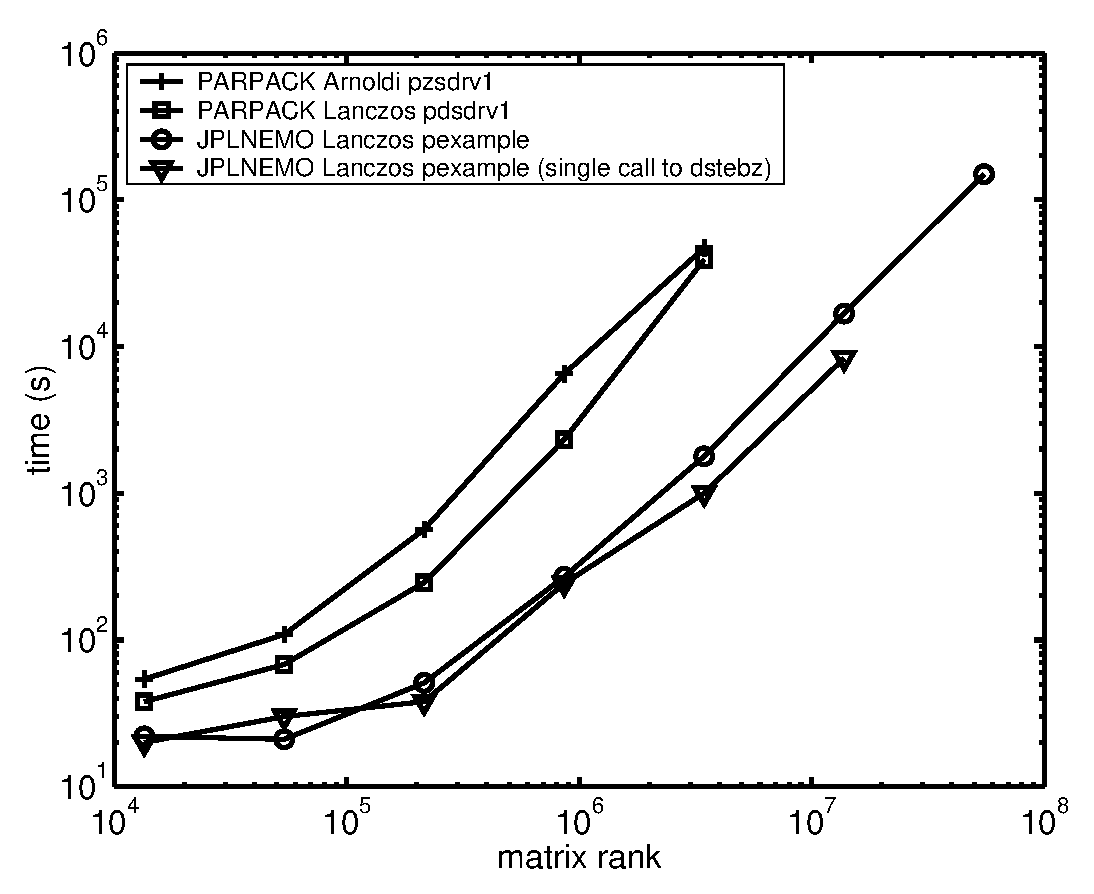
\includegraphics[width=80mm, height=60mm]{fig1.eps}
    		\end{minipage}
    		\hspace{.04\textwidth}
   		\begin{minipage}{.45\textwidth}
      			\centering
      			\caption{Performance comparison of solution of test
problem between two different PARPACK solvers and JPLNEMO-Lanczos.}
			\label{fig:compare}
    		\end{minipage}
	  	\vspace{3mm}
  	\end{figure}

The results of the experiments are shown in Figure~\ref{fig:compare}.  
The JPL NEMO Lanczos eigensolver
ran roughly 20 times faster than the PARPACK Lanczos eigensolver
using about 20 times less memory.  This can make a significant difference
in the eigensystem problem size that can be solved
in a limited amount of time with a limited amount of system memory.
Both ARPACK and JPL NEMO eigensolvers report
the total number of matrix-vector multiplications required.
The ARPACK eigensolvers always required about twice as many
matrix-vector multiplication in these experiments.
For all problem sizes except the largest,
the JPL NEMO eigensolver ran almost as fast
with one call to Fortran~77 {\tt subroutine dstebz} every $100$ iterations
as it did with just one call at the end of the Lanczos iterations,
so that checking for convergence every 100 iterations does not
introduce significant overhead.

\subsubsection{Speedup}

	\begin{figure}[t]
		\vspace{4mm}
    		\begin{minipage}{.5\textwidth}
      			\centering
      			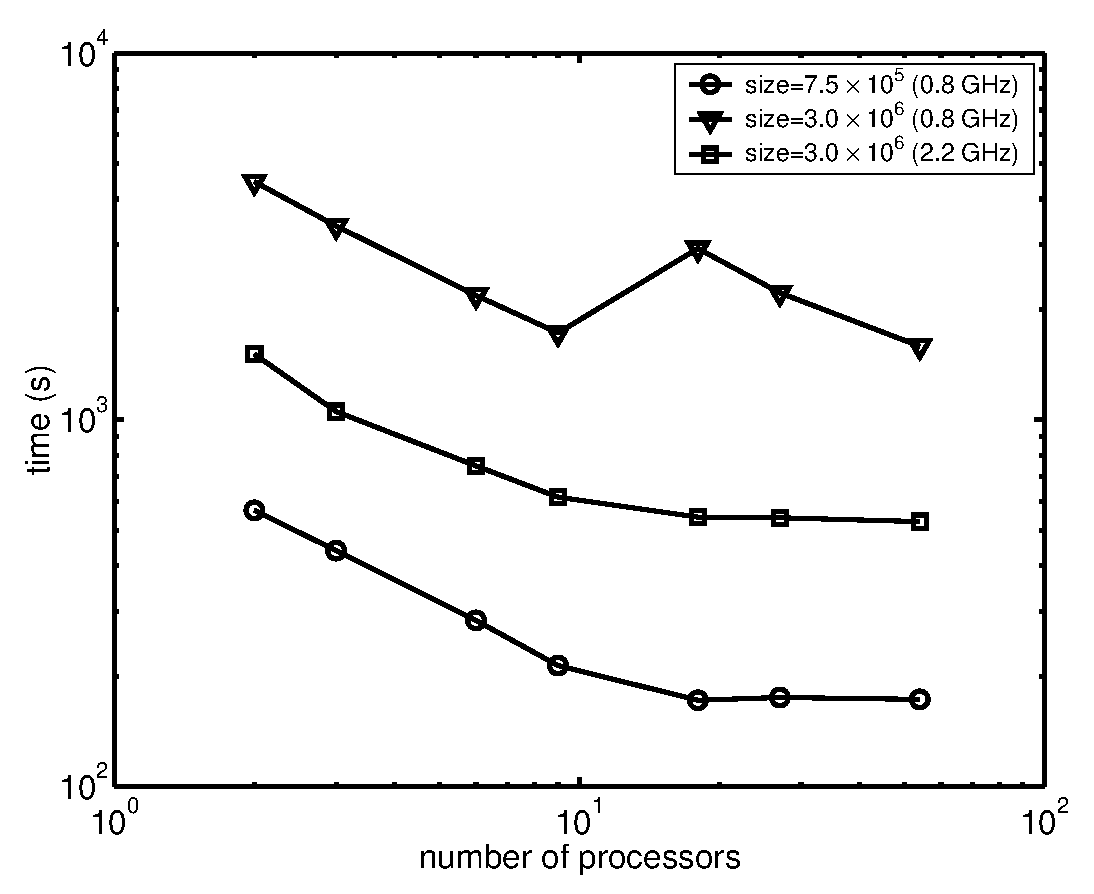
\includegraphics[width=80mm, height=60mm]{fig2.eps}
    		\end{minipage}
    		\hspace{.04\textwidth}
   		\begin{minipage}{.45\textwidth}
      			\centering
      			\caption{Wall time for test problem of two sizes ($7.5 \times 10^5$ and $3.0 \times 10^6$).  The early onset of saturation of speedup is likely due to the low cost of computation relative to communication for the test linear operator.}
			\label{fig:speedup}
    		\end{minipage}
	  	\vspace{3mm}
  	\end{figure}

Experiments were conducted with the JPL NEMO eigensolver
for two small problem sizes (matrices of rank $746,496$ and $2,985,985$)
on $2$, $3$, $6$, $9$, $18$, $27$ and $54$ processors to measure speedup.
The $2,985,985$ diagonal element experiment was repeated
on a Beowulf cluster with 66 nodes of dual $2200$MHz Intel Xeon processors
with $512$KByte cache, $2$GByte shared system memory
and a fast ethernet switch running MPICH 1.2.4 under Red Hat Linux 7.3.
The results are shown in Figure~\ref{fig:speedup}.
We expect diminishing returns in speedup for small problem sizes
as the Lanczos vectors are diluted among an increasing number of processors.
We also expect network congestion to be a problem
because all of the processors attempt to communicate at the same time.
Performance does not always degraded gracefully.
Increasing the number of processors can actually increase execution time
as it does for $9$ and $18$ processors on our $800$MHz Beowulf cluster.
It appears that efficiency is maximized at about $10$ processors on simple,
small problems and adding more processors may actually reduce performance.

\section{Conclusions}
The JPL NEMO Lanczos eigensolver
for large, sparse complex Hermitian eigensystems
is much faster and requires much less memory
than comparable PARPACK eigensolvers
and may have an advantage over the PARPACK eigensolvers
in applications where it isn't necessary to obtain
all of the eigenvalues in a particular range or
where multiplicity is unimportant.
The difference in performance and efficiency
is attributed to a more simple and straight-forward implementation
of the Lanczos algorithm in the JPL NEMO eigensolver
than in the more robust and sophisticated PARPACK eigensolvers.

The JPL NEMO and PARPACK eigensolvers were compared using
a simple real symmetric eigensystem in order to minimize
the time required to perform the matrix-vector multiplication.
In realistic applications where the eigensystem is nontrivial,
the matrix-vector multiplication may actually dominate
the total execution time of both JPL NEMO and PARPACK eigensolvers
but we would still expect the JPL NEMO eigensolver
to be at least twice as fast if the PARPACK eigensolvers required
twice as many matrix-vector multiplications.

For the simple linear operator described in section~\ref{sec:cmp},
using more than about a dozen processors does not help speed up
the JPL NEMO eigensolver benchmark very much
as communication time begins to dominate total execution time
for simple eigensystems and small problem sizes.
Clearly, increasing ratio of computation to communication
would lead to a less pronounced saturation of speedup
with the number of processors.

% Experience with more realistic eigensystems
% where the ratio of computation to communication is higher
% in the matrix-vector multiplication seems to indicate
% that more processors can increase speedup.

\section{Acknowledgments}
The original author of the JPL NEMO eigensolver software
was Chris Bowen with Texas Instruments in Dallas, Texas
who is a former employee at the Jet Propulsion Laboratory
in Pasadena California.
Richard Lehoucq at Sandia National Labs contributed
to the design of a fair comparison of the JPL NEMO eigensolver
with PARPACK eigensolvers
through many thoughtful electronic mail messages.
David J.C. MacKay with the Cavendish Laboratory in Cambridge, England
 wrote the MACOPT optimizer package
and release it under the GNU Lesser General Public License (LGPL)
so that we code modify his code and distribute it
with the JPL NEMO eigensolver under the LGPL.

\appendix
\section{Installation}
The JPL NEMO Lanczos eigensolver package
is distributed as a compressed UNIX tape archive {\tt eigen.tgz}
though the Channel Foundation at
\begin{verbatim}
http://www.openchannelsoftware.com/
\end{verbatim}
It includes a copy of the JPL NEMO Math Library (NML) and
the Linear Algebra PACKage (LAPACK) library.
It requires a C or C++ compiler
and the the Message Passing Interface (MPI) package.
A Fortran~77 compiler may also be required to compile the LAPACK library
or the example program.
The JPL NEMO Lanczos eigensolver package distribution
is configured to install under Red Hat Linux, 7.3
using MPICH and the GNU tool chain by default
but it is easily reconfigured to install on any UNIX platform.
It compiles under Red Hat Linux 8.0, IRIX64 6.5 and Mac OS X 10.2
here at the Jet Propulsion Laboratory.

Typical users should be able
to download the JPL NEMO Lanczos eigensolver package {\tt eigen.tgz}
into their home directory and install it by simply typing
\begin{verbatim}
        $ tar xvzf eigen.tgz
        $ cd eigen
        $ make
        $ cd examples
        $ make
\end{verbatim}
then run the parallel example program by simply typing
\begin{verbatim}
        $ run
\end{verbatim}
at their UNIX prompt {\tt \$}.
Atypical users should not despair.

The default installation configuration uses environment variables
\begin{center}
\begin{tabular}{l|l}
variable	&description		\\
\hline
{\tt MPI\_HOME}	&MPI home directory and	\\
{\tt HOSTTYPE}	&UNIX host type.
\end{tabular}
\end{center}
The GNU {\tt make} program uses {\tt eigen/Makefile}
to build the JPL NEMO eigensolver package.
This Makefile defines just a few important variables:
\begin{center}
\begin{tabular}{l|l|l}
variable	&default value			&description		\\
\hline
{\tt PLATFORM}	&{\tt \$(HOSTTYPE)}		& platform		\\
{\tt CC}	&{\tt \$(MPI\_HOME)/bin/mpiCC}	& MPI C or C++ compiler	\\
{\tt LD}	&{\tt \$(MPI\_HOME)/bin/mpiCC}	& MPI link editor	\\
{\tt DEFINES}	&{\tt -DNML\_ERRANT}	& NML cpp macros definitions	\\
{\tt OPTIONS}	&{\tt -O2 -Wall -ansi -pedantic}& NML C or C++ options	\\
{\tt FORTRAN}	&{\tt /usr/bin/f77}		& LAPACK Fortran compiler\\
{\tt OPTS}	&{\tt -funroll-all-loops -fno-f2c -O3}& LAPACK Fortran options\\
{\tt BLASLIB}	&{\tt blas\_\$(PLATFORM).a}	& BLAS library archive	\\
{\tt LAPACKLIB}	&{\tt lapack\_\$(PLATFORM).a}	& LAPACK library archive\\
{\tt CCMKD}	&{\tt /usr/bin/g++ -MM}	& eigen make dependencies	\\
{\tt CCOPT}	&{\tt -Wall -O3 -DFORTRAN\_UNDERSCORE}& eigen C or C++ options
\end{tabular}
\end{center}
Users can override these variable definitions
by editing the Makefile or through {\tt make} command line arguments
\begin{verbatim}
make PLATFORM=powerpc
\end{verbatim}
for example.
The platform variable should be a unique name
which specifies the particular combination
of computer architecture, operating system, compiler, library, etc.
used to build the JPL NEMO eigensolver library.
It is used to create directories for run-time library archives
that co-exist for each of several different platforms
that might remote mount the user's file system

The {\tt make} program descends into directories
{\tt eigen/LAPACK}, {\tt eigen/nml} and {\tt eigen/src}
and invokes {\tt make} with the appropriate overriding variables,
so normally there should be no reason to modify any of the makefiles
in these directories.

The JPL NEMO eigensolver package requires
\begin{center}
\begin{tabular}{l|l}
archive						& description		\\
\hline
{\tt eigen/LAPACK/blas\_\$PLATFORM.a}	& BLAS run-time library,	\\
{\tt eigen/LAPACK/lapack\_\$PLATFORM.a}	& LAPACK run-time library,	\\
{\tt eigen/nml/include/\$PLATFORM/}	& NML compile-time library and	\\
{\tt eigen/nml/lib/\$PLATFORM/}		& NML run-time library.
\end{tabular}
\end{center}
Users who have already installed LAPACK or NML
and wish to use their existing libraries
instead of building the LAPACK or NML libraries
distributed with the the JPL NEMO eigensolver
can do so by simply by removing directories
{\tt eigen/LAPACK} and {\tt eigen/nml}
and substituting links to the existing installations.

The {\tt eigen/examples/} directory contains a shell script
\begin{verbatim}
run [processors [blocks [values [maxitr]]]]
\end{verbatim}
which can be used to invoke {\tt mpirun} with the parallel example program
{\tt pexample} and options specifying the number of processors,
the number of blocks in the real symmetric block tridiagonal matrix $A$,
the number of eigenvalues requested and the maximum number of iterations.
The {\tt eigen/examples/parpack/} directory
contains the PARPACK Fortran 77 programs used in the comparison
with the JPL NEMO eigensolver.

\section{The JPL NEMO Math Library (NML)}\label{app:nml}
This appendix describes the data structures and associated methods
contained within the JPL NEMO Math Library, an open software replacement
for the proprietary vector and matrix types
provided with Numerical Recipes in C\cite{press}.
The {\tt nml\_} and {\tt NML\_} prefixes are reserved
for NML type and function names.
There are four implementation dependent type definitions:
\begin{center}
\begin{tabular}{c|r|l}
superset&	definition	&synonym		\\
\hline
cardinal&	{\tt size\_t}	&{\tt nml\_extent}	\\
cardinal&	{\tt size\_t}	&{\tt nml\_offset}	\\
integral&	{\tt ptrdiff\_t}&{\tt nml\_stride}	\\
integral&	{\tt ptrdiff\_t}&{\tt nml\_index}
\end{tabular}
\end{center}

All other NML type names are formed by the {\tt nml\_} prefix
followed by three fields {\tt nml\_<p><s><basetype>}.

There are four [finite] precision arithmetics:
\begin{center}
\begin{tabular}{c|l|r|l}
{\tt <p>}& {\tt <precision>}&definition&	\\
\hline
{\tt d}&   {\tt double}	&{\tt double}  &double precision floating-point	\\
{\tt s}&   {\tt single}	&{\tt float}   &single precision floating-point	\\
{\tt i}&   {\tt integer}&{\tt   signed int}&integral	\\
{\tt l}&   {\tt logical}&{\tt unsigned int}&boolean
\end{tabular}
\end{center}

There are two number systems:
\begin{center}
\begin{tabular}{c|c|l}
{\tt <s>}	&{\tt <system>}	&definition				\\
\hline
{\tt c}		&{\tt complex}	&Cartesian complex number system	\\
		&		&real number system
\end{tabular}
\end{center}

There are eight base types:
\begin{center}
\begin{tabular}{c|c|c|l}
	&			&index		&			\\
{\tt <b>}&{\tt <basetype>}	&base		&description		\\
\hline
{\tt s}&{\tt scalar}		&		&scalar			\\
{\tt v}&{\tt vector}		&$0$		&vector			\\
{\tt m}&{\tt matrix}		&$0$		&matrix			\\
{\tt t}&{\tt tensor}		&$0$		&tensor			\\
\hline
{\tt 1D}&{\tt 1DBase}		&arbitrary	&vector			\\
{\tt 2D}&{\tt 2DBase}		&arbitrary	&matrix			\\
{\tt 3D}&{\tt 3DBase}		&arbitrary	&tensor			\\
\hline
{\tt 3}&{\tt 3bands}		&$0$		&tridiagonal matrix
\end{tabular}
\end{center}

There are additional synonyms for scalars:
\begin{center}
\begin{tabular}{l|l|l}
\hline
{\tt nml\_<p>scalar}	&{\tt nml\_<precision>}	&real		\\
{\tt nml\_<p>cscalar}	&{\tt nml\_<p>complex}	&complex	\\
\hline
\end{tabular}
\end{center}

All NML function names are prefixed with {\tt nml\_<p><s><b>\_}
where {\tt <b>} is an abbreviation for the {\tt <basetype>}.
Memory for vector, matrix and tensor types is allocated from free storage
and these objects are always referenced only through pointers.
This permits access to the individual elements of a vector, matrix
or tensor object using the ordinary C subscript operator[].

There are two pseudo-constructors,
\begin{enumerate}
\item	{\tt new}   constructs uninitialized objects from their extents and
\item	{\tt clone} constructs a copy of an existing object of the same type.
\end{enumerate}
The destructor {\tt delete} deallocates any storage allocated for an object.
The reconstructor {\tt resize} {\tt delete}'s an object
then replaces it with a new uninitialized object with the specified extents.
Extents appear in reverse order from right to left in the argument list
of {\tt new} and {\tt resize} just as they do in the subscript operators.
Function {\tt extent1} returns the rightmost extent
from two and three dimensional objects.
Of course, vector and tridiagonal matrix objects have just one extent
which may be retrieved by function {\tt extent}.

\begin{center}
\begin{tabular}{r|c|l}
object		&return type
&pseudo-constructor	\\
\hline
		      $n$ vector&{\tt nml\_<p><s>vector*}
&{\tt nml\_<p><s>v\_new(n)} \\
	  $m\!\times\!n$ matrix &{\tt nml\_<p><s>matrix*}
&{\tt nml\_<p><s>m\_new(m, n)} \\
$l\!\times\!m\!\times\!n$ tensor&{\tt nml\_<p><s>tensor*}
&{\tt nml\_<p><s>t\_new(l, m, n)} \\
\end{tabular}
\end{center}

\begin{center}
\begin{tabular}{r|c|l}
return type	&pseudo-constructor	&argument type	\\
\hline
{\tt nml\_<p><s>vector*}&{\tt nml\_<p><s>v\_clone(v)}
&{const \tt nml\_<p><s>vector* v} \\
{\tt nml\_<p><s>matrix*}&{\tt nml\_<p><s>m\_clone(M)}
&{const \tt nml\_<p><s>matrix* M} \\
{\tt nml\_<p><s>tensor*}&{\tt nml\_<p><s>t\_clone(T)}
&{const \tt nml\_<p><s>tensor* T} \\
\end{tabular}
\end{center}

\begin{center}
\begin{tabular}{r|l|c}
				returns&re-constructor
&argument type		\\
\hline
		      $n$ vector {\tt *pv}
&{\tt nml\_<p><s>v\_resize(pv, n)}	&{\tt nml\_<p><s>vector** pv} \\
	   $m\!\times\!n$ matrix {\tt *pM}
&{\tt nml\_<p><s>m\_resize(pM, m, n)}	&{\tt nml\_<p><s>matrix** pM} \\
$l\!\times\!m\!\times\!n$ tensor {\tt *pT}
&{\tt nml\_<p><s>t\_resize(pT, l, m, n)}&{\tt nml\_<p><s>tensor** pT}
\end{tabular}
\end{center}

\begin{center}
\begin{tabular}{c|c}
destructor			&argument type			\\
\hline
{\tt nml\_<p><s>v\_delete(v)}	&{\tt nml\_<p><s>vector* v}	\\
{\tt nml\_<p><s>m\_delete(M)}	&{\tt nml\_<p><s>matrix* M}	\\
{\tt nml\_<p><s>t\_delete(T)}	&{\tt nml\_<p><s>tensor* T}
\end{tabular}
\end{center}

\begin{center}
\begin{tabular}{c|c|c}
vector
&matrix				&tensor				\\
\hline
 {\tt nml\_<p><s>v\_extent(v)}
&{\tt nml\_<p><s>m\_extent1(M)}	&{\tt nml\_<p><s>t\_extent1(T)}	\\
&{\tt nml\_<p><s>m\_extent2(M)} &{\tt nml\_<p><s>t\_extent2(T)}	\\
&				&{\tt nml\_<p><s>t\_extent3(T)}
\end{tabular}
\end{center}

There are vector-scalar operations:
\begin{center}
\begin{tabular}{c|l|l}
{\tt nml\_<p><s>v\_fill(v, x)} &$v_{j} \leftarrow x$&$0 \leq j < n$	      \\
{\tt nml\_<p><s>v\_smul(v, x)} &$v_{j} \leftarrow v_{j}\cdot x$&$0 \leq j < n$\\
{\tt nml\_<p><s>v\_sdiv(v, x)} &$v_{j} \leftarrow v_{j}/x$&$0 \leq j < n$     \\
{\tt nml\_<p><s>v\_sadd(v, x)} &$v_{j} \leftarrow v_{j} + x$&$0 \leq j < n$   \\
{\tt nml\_<p><s>v\_ssub(v, x)} &$v_{j} \leftarrow v_{j} - x$&$0 \leq j < n$
\end{tabular}
\end{center}
which return a pointer to the first element of vector $v$.

There are vector reduction operations:
% \begin{center}
\begin{center}
\begin{tabular}{l|l}
{\tt nml\_<p><s>v\_ssqr(v)}	&$\sum_{j\!=\!0}^{n\!-\!1} v_{j}^{2}$	\\
									\\
{\tt nml\_<p><s>v\_sabs(v)}	&$\sqrt{\sum_{j\!=\!0}^{n\!-\!1} v_{j}^{2}}$
\end{tabular}
\end{center}
and
% \begin{center}
\begin{center}
\begin{tabular}{l|c|l}
{\tt nml\_<p><s>v\_sminmag(v)}&$\mbox{min}\{||v_{j}||\}$&$0 \leq j < n$	\\
{\tt nml\_<p><s>v\_smaxmag(v)}&$\mbox{max}\{||v_{j}||\}$&$0 \leq j < n$	\\
\end{tabular}
\end{center}
which return a real scalar {\tt nml\_<p>scalar}.

There are vector-vector operations:
\begin{center}
\begin{tabular}{c|l|l}
{\tt nml\_<p><s>v\_vcpy(v, w)}&$v_{j} \leftarrow w_{j}$&$0 \leq j < n$	      \\
{\tt nml\_<p><s>v\_vmul(v, w)}&$v_{j} \leftarrow v_{j}\cdot w_{j}$&$0 \leq j < n$\\
{\tt nml\_<p><s>v\_vdiv(v, w)}&$v_{j} \leftarrow v_{j}/w_{j}$&$0 \leq j < n$  \\
{\tt nml\_<p><s>v\_vadd(v, w)}&$v_{j} \leftarrow v_{j} + w_{j}$&$0 \leq j < n$\\
{\tt nml\_<p><s>v\_vsub(v, w)}&$v_{j} \leftarrow v_{j} - w_{j}$&$0 \leq j < n$
\end{tabular}
\end{center}
which return a pointer to the first element of vector $v$.

% \begin{center}
% \begin{tabular}
% \end{tabular}
% \end{center}

%\nocite{ARPACK, press, golub, trefethen, yang:99, wusi:99, www:arpack}
\bibliography{lanczos}

\end{document}

